\section{Process View} \label{design:processView}

\todo{Re-read this because I was pretty tired as I corrected this shit}

Previously we broke down the requirements for the functionality of the bus into a number of components, and created a class diagram \ref{fig:softwareArchitecture} to structure how those would interact. The next step is to create interfaces and thereby clear, concrete contracts of the intended functionality of each major class in the program. 

In non real-time systems the class and system structure may be enough to start creating interfaces, but in this case we still need to figure out we will reconcile the class structure with the chosen scheduling method. As mentioned in \ref{analysis:scheduling}, we will be using fixed priority scheduling\todo{With or without preemption?} to decide when the tasks in the bus are run. One of the questions that we need to clear up in this regard is where we run the program from and where the main function resides. %Specifically, where are the components initialised and where do we ensure that they deliver their data to the correct receiver? Besides answering these questions, we must ensure that conventions of good object-oriented design are still followed. Specifically, the trouble is keeping a low coupling between the components, even though they all need to communicate with the driving-component. 

\subsubsection{Program Flow}
The program flow and main function is defined within the .oil-files; see a description of these in section \ref{OILteo}. Inside the .oil-files we define functions as tasks which will be called with specific priorities, periods and deadlines. 

The \code{ObstacleDetection}-component (which uses the ultrasonic sensor to check for obstacles ahead of the vehicle) will be used as an example to illustrate the issue. If the program did not have to be a real-time system, then the obvious solution would simply be to detect obstacles regularly. If any are found, then the Driving-component is immediately alerted, which then calls the motor controls and adjust the direction of the bus.

The issue in this case is that the bus might miss a lot of other deadlines while the Driving-component has control of the CPU. This is of course unacceptable, because, depending on the circumstances, the bus might no longer meet its other requirements. 

Imagine the following worst case. The bus detects a bus stop and decides to park there. Now the driving component gains control of the CPU for the next two seconds while it parks the bus. All deadlines are lost in that time, and if there's an obstruction on the road that was not detected prior, it might not be detected until it is too late.

The solution to this is splitting the above task into separate, smaller tasks: sensor detection and the execution of driving commands. Both of these are then be scheduled and executed entirely independently. This means that the system might wait longer before executing a stop-command. However, this should not be a problem, as long as we ensure that the period is short enough, so that the bus can always stop in time before crashing into something. 

This works by having the .oil-files call the individual components as often as necessary, which then return their result or suggested steering response (continue driving, brake, turn left, etc.) to the Driving-component. The driving component is then called at a separate time to decide which command to execute and then do so.

The Driving-component now handles everything in regards to input and output of the different components, and also deals with prioritising the steering commands, to figure out what the motor should actually do if there is any ambiguity (imagine it both found a bus stop and an obstruction in the road). 

Imagine a case where the scheduler first selects the \code{ObstacleDetection}-component to control the CPU, and an obstacle is detected, and the car is stopped. See the sequence diagram in figure \ref{fig:sequenceDetectObstacle} for how the program flow would look.

\begin{figure}[ht]
    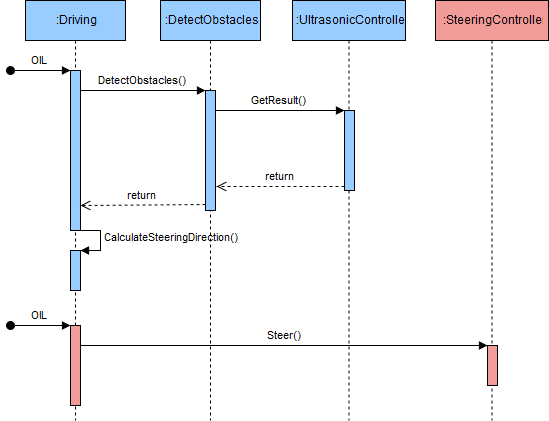
\includegraphics[width=\textwidth]{Images/Design/sequenceObstacleDetection.png}
    \caption{Sequence diagram showing the program flow while detecting obstacles and reacting to this.}
    \label{fig:sequenceDetectObstacle}
\end{figure}

s\todo{From supervisor: This communication can be through shared variable(s): e.g. obstacle detector is being run periodically and then marks some variables that there is some obstacle somewhere, then the driver could be running at its own pace and check the obstable variables.
It is not clear how/why do you actually structure/map classes to tasks and how/why things are connected.
In this picture it is clear that communication between classes are synchronous function/method calls, but it does not neccessarily have to be this way.
It seems that you are not exploiting (pseudo)parallelism and your tasks seem sequential (one after another).}

Task A calls the \code{ObstacleDetection}-component, which then returns results from the ultrasonic sensor. At this point the control is returned to the scheduler, which uses the .oil file to decide which tasks receives control next. 

At some point later (there may have been other tasks run in the meantime) task B is scheduled to run. Task B then assigns control of the CPU to the driving component again, which decides based on the data that it received how it should steer the bus in response. In this case, because the \code{ObstacleDetection}-component returns data that there is an obstacle on the road, the \code{Driving}-component will respond by braking the car\todo{Couldn't this be done with a quick command instead? "motor speed = 0", no need to have the driving component to do this. Answer: yes it can, but it's just a bad idea because of the problem outlined with the BusStop command. We want each task to have clear boundaries on what it may do. They don't mess directly with the sensors; the driving component does this.}. Task B is fully separate from obstacle detection, and regardless of which task was executed prior, task B just executes the top priority command. 




\todo{Oprems ALLE tasks. Skriv også om vores TaskMain, som har prioritet på 1, men startes først, og har en uendelig while løkke hvor programmet busy-waiter hvis ikke det ellers kører andre tasks. Kunne man have gjort det på en anden måde? }